% Asset ID: AS1ExponentialsAndLogarithmsTikZ-004
% Asset type: TikZ diagram
% Suggested file path: tikz/AS1ExponentialsAndLogarithmsTikZ-004.tex
% Unit code: AS1
% Topic code: AS1-EXPLOG
% Topic name: Exponentials and logarithms
% Related lesson section: Core Theory 7; Worked Example 4
% Source: Chapter 14 PDF; CCEA AS1-EXPLOG simple transformations of e^x
% Purpose: Show y = e^x and y = 2 + e^(x/3), including shifted horizontal asymptote y = 2.
\documentclass[tikz,border=8pt]{standalone}
\usepackage{amsmath}
\usepackage{pgfplots}
\pgfplotsset{compat=1.18}
\begin{document}
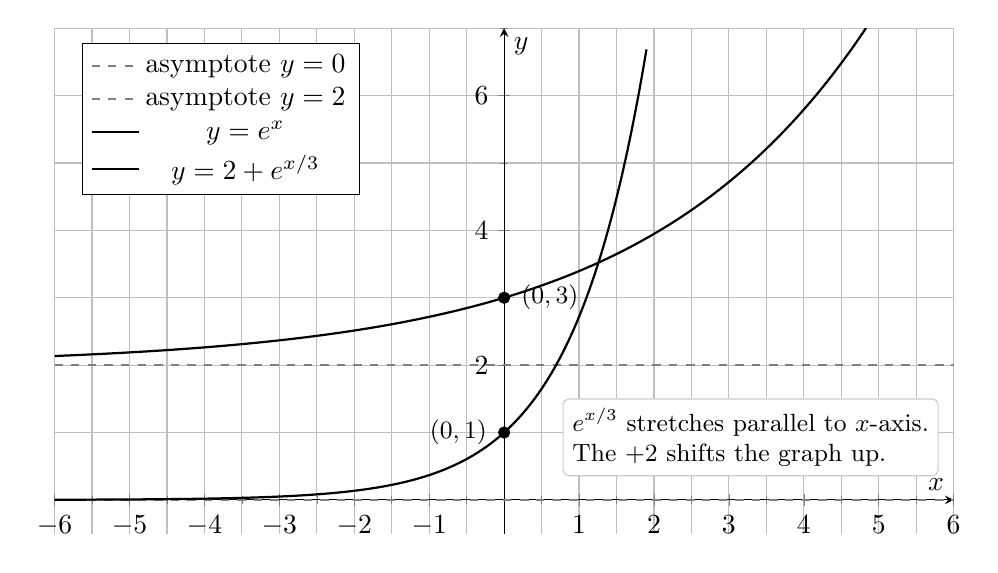
\begin{tikzpicture}
\begin{axis}[width=13cm,height=8cm,axis lines=middle,xmin=-6,xmax=6,ymin=-0.5,ymax=7,xlabel={$x$},ylabel={$y$},grid=both,minor tick num=1,samples=250,legend pos=north west]
\addplot[dashed,thick,gray,domain=-6:6]{0};\addlegendentry{asymptote $y=0$}
\addplot[dashed,thick,gray,domain=-6:6]{2};\addlegendentry{asymptote $y=2$}
\addplot[thick,domain=-6:1.9]{exp(x)};\addlegendentry{$y=e^x$}
\addplot[thick,domain=-6:5.2]{2 + exp(x/3)};\addlegendentry{$y=2+e^{x/3}$}
\addplot[only marks,mark=*,mark size=2pt] coordinates {(0,1) (0,3)};
\node[anchor=east,font=\small] at (axis cs:-0.1,1) {$(0,1)$};
\node[anchor=west,font=\small] at (axis cs:0.1,3) {$(0,3)$};
\node[align=left,anchor=south east,font=\small,fill=white,draw=black!20,rounded corners=2pt] at (axis cs:5.8,0.35) {$e^{x/3}$ stretches parallel to $x$-axis.\\The $+2$ shifts the graph up.};
\end{axis}
\end{tikzpicture}
\end{document}
